\section{Shift Registers}
\label{sec:shift-registers}

A register capable of shifting the binary information held in each cell to its neighboring cell, in a selected direction, is called a \textit{shift register}.
The simplest possible shift register is one that uses only flip-flops, as shown in Fig. 3.
\begin{figure}[H]
  \centering
  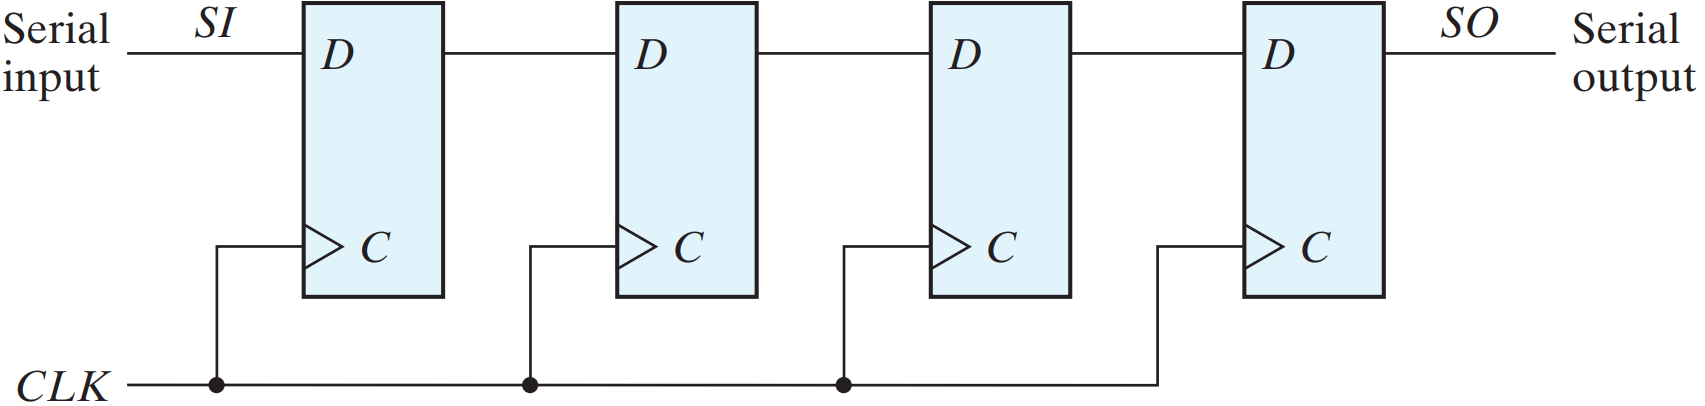
\includegraphics[width=\linewidth]{img/fig-6.3.png}
  \caption{Four-bit shift register}
  \label{fig:6.3}
\end{figure}
\noindent This shift register is unidirectional (left-to-right). Each clock pulse shifts the contents of the register one bit position to the right.

\subsection{Serial Transfer}
\label{subsec:serial-transfer}

The datapath of a digital system is said to operate in serial mode when \textit{information is transferred and manipulated one bit at a time}. The serial transfer of information from register $A$ to register $B$ is done with shift registers, as shown in the block diagram of Fig. 6.4(a).
\begin{figure}[H]
  \centering
  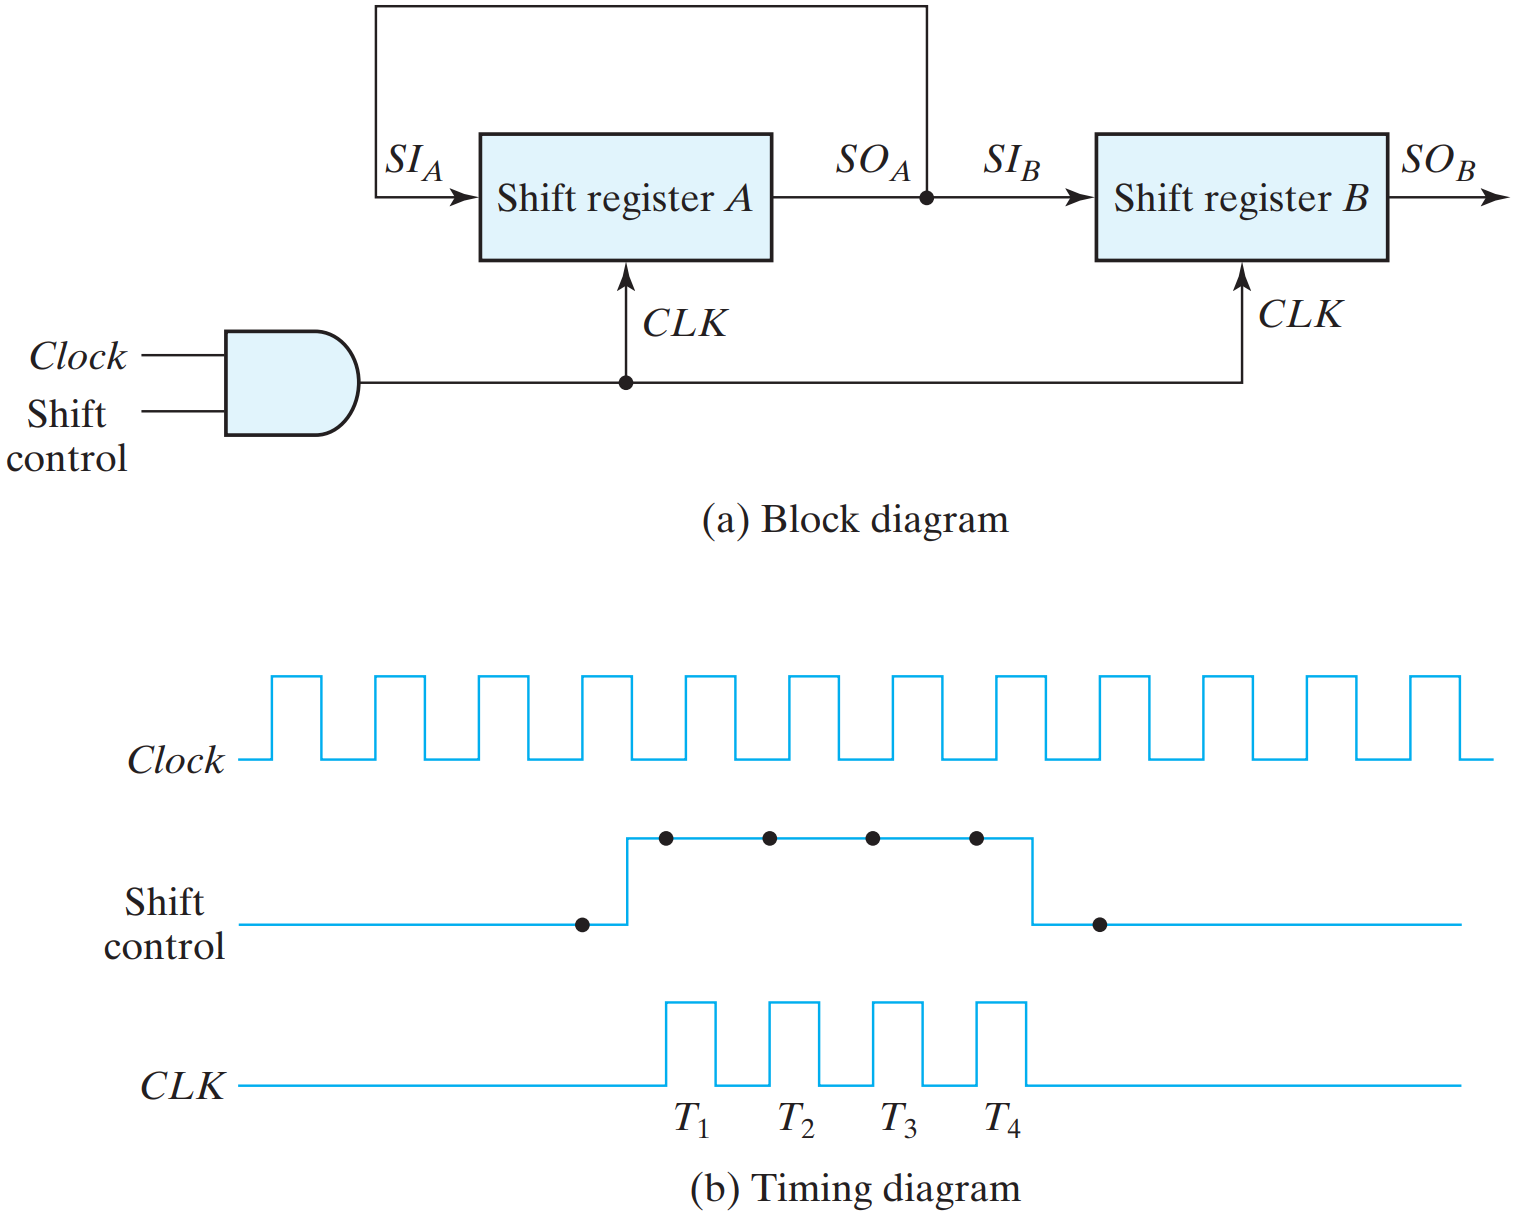
\includegraphics[width=\linewidth]{img/fig-6.4.png}
  \caption{Serial transfer from register $A$ to register $B$}
  \label{fig:6.4}
\end{figure}
\noindent Four pulses: $T_1$, $T_2$, $T_3$, and $T_4$. Each rising edge of the pulse causes a shift in both registers.
\begin{figure}[H]
  \centering
  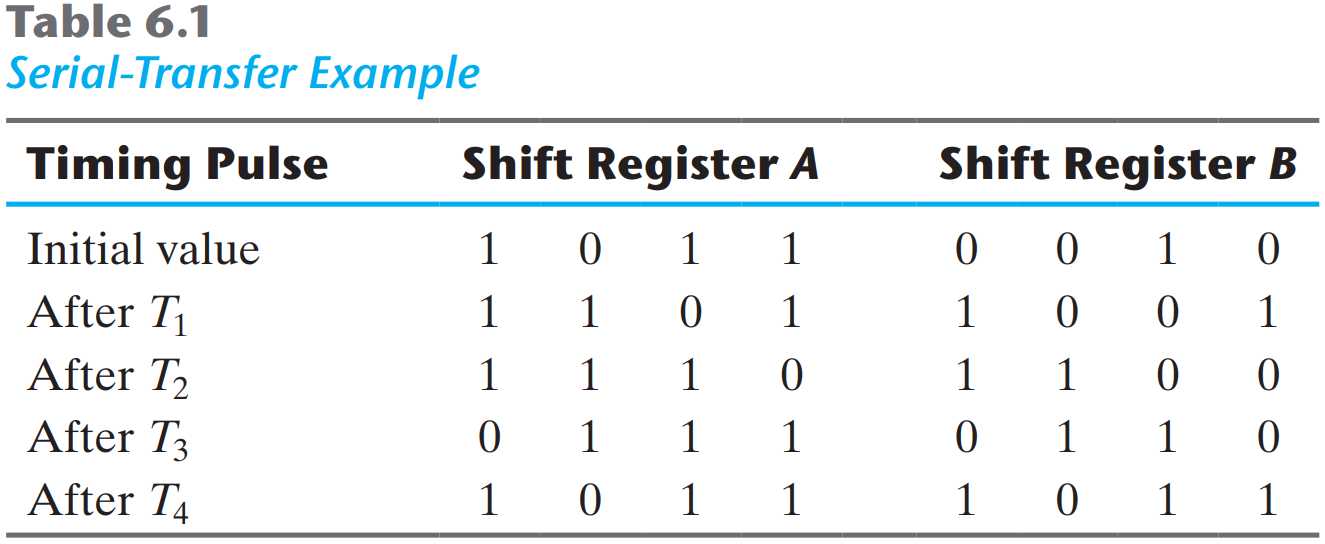
\includegraphics[width=\linewidth]{img/table-6.1.png}
  \label{table:6.1}
\end{figure}

One application of shift registers is converting between ``serial data'' and ``parallel data''. Computers typically work with multiple-bit quantities (ASCII: 8 bits long; Integers: 32 bits long.). But sometimes it's necessary to send or receive data serially, or one bit at a time. Some examples includes: Input devices such as keyboards and mice or output devices like printers.

\noindent Receiving serial data:
\begin{figure}[H]
  \centering
  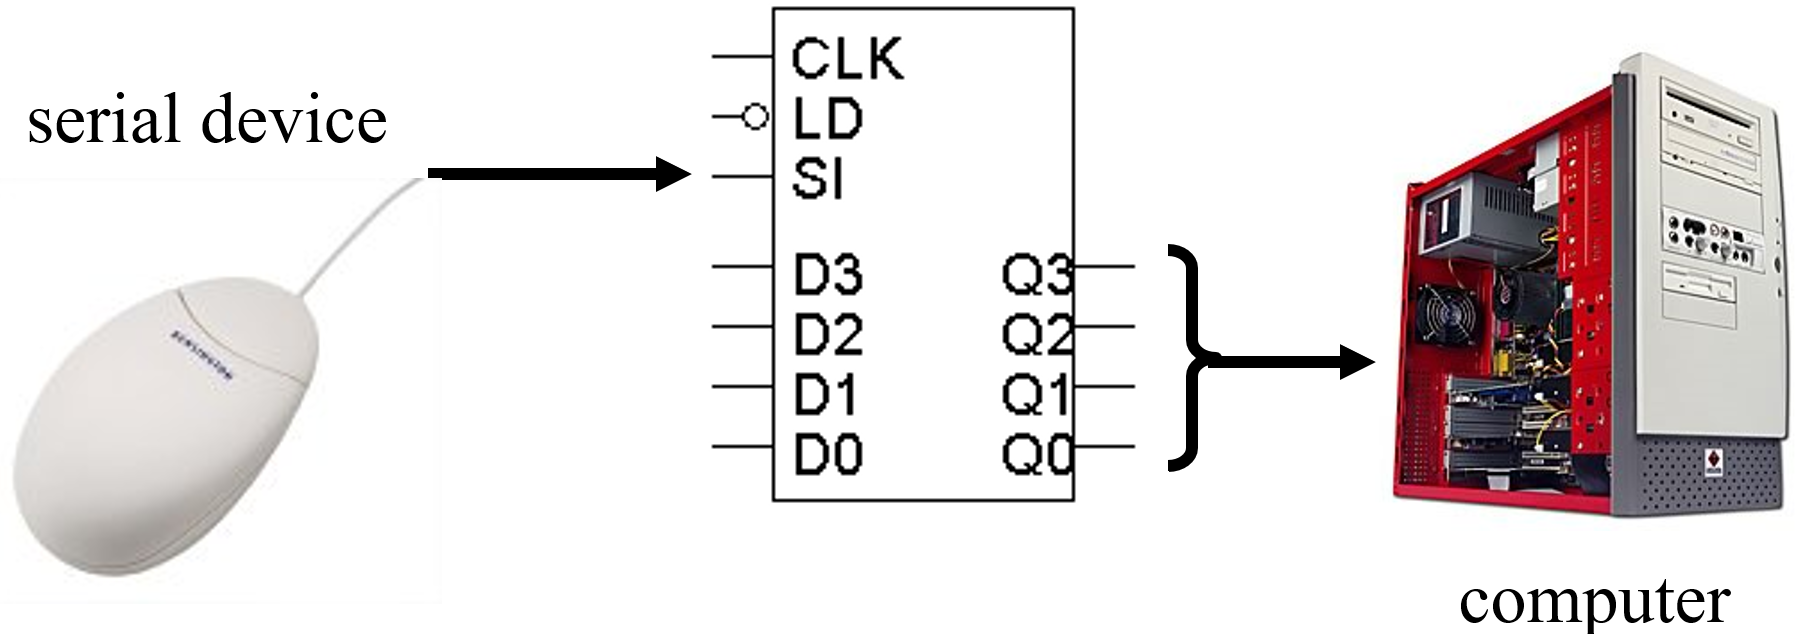
\includegraphics[width=\linewidth]{img/receiving-serial-data.png}
\end{figure}
\noindent Sending data serially:
\begin{figure}[H]
  \centering
  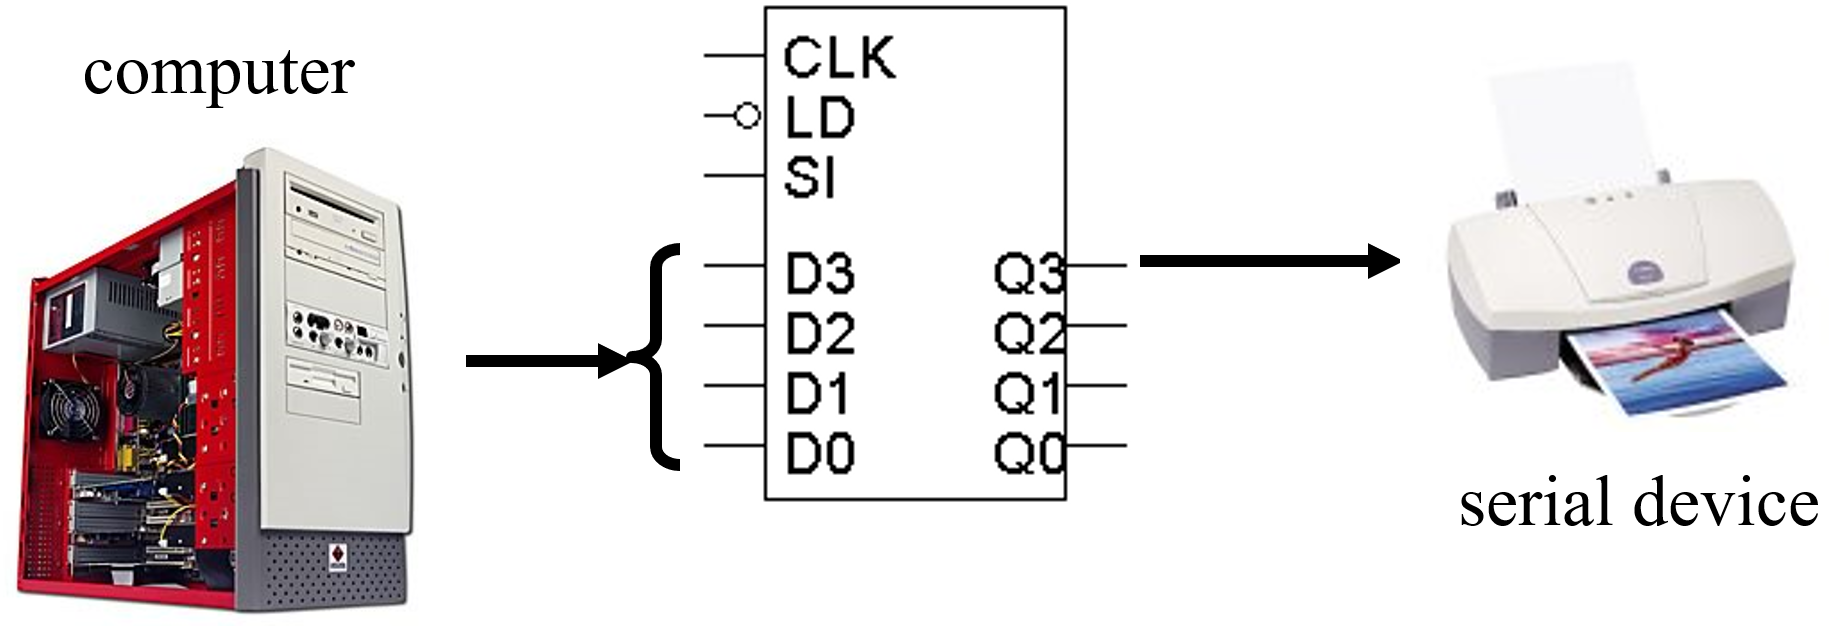
\includegraphics[width=\linewidth]{img/sending-data-serially.png}
\end{figure}

\subsection{Serial Addition}
\label{subsec:serial-addition}

The two binary numbers to be added serially are stored in two shift registers. Beginning with the least significant pair of bits, the circuit adds one pair at a time through a single full-adder (FA) circuit, as shown in Fig. 5.
\begin{figure}[H]
  \centering
  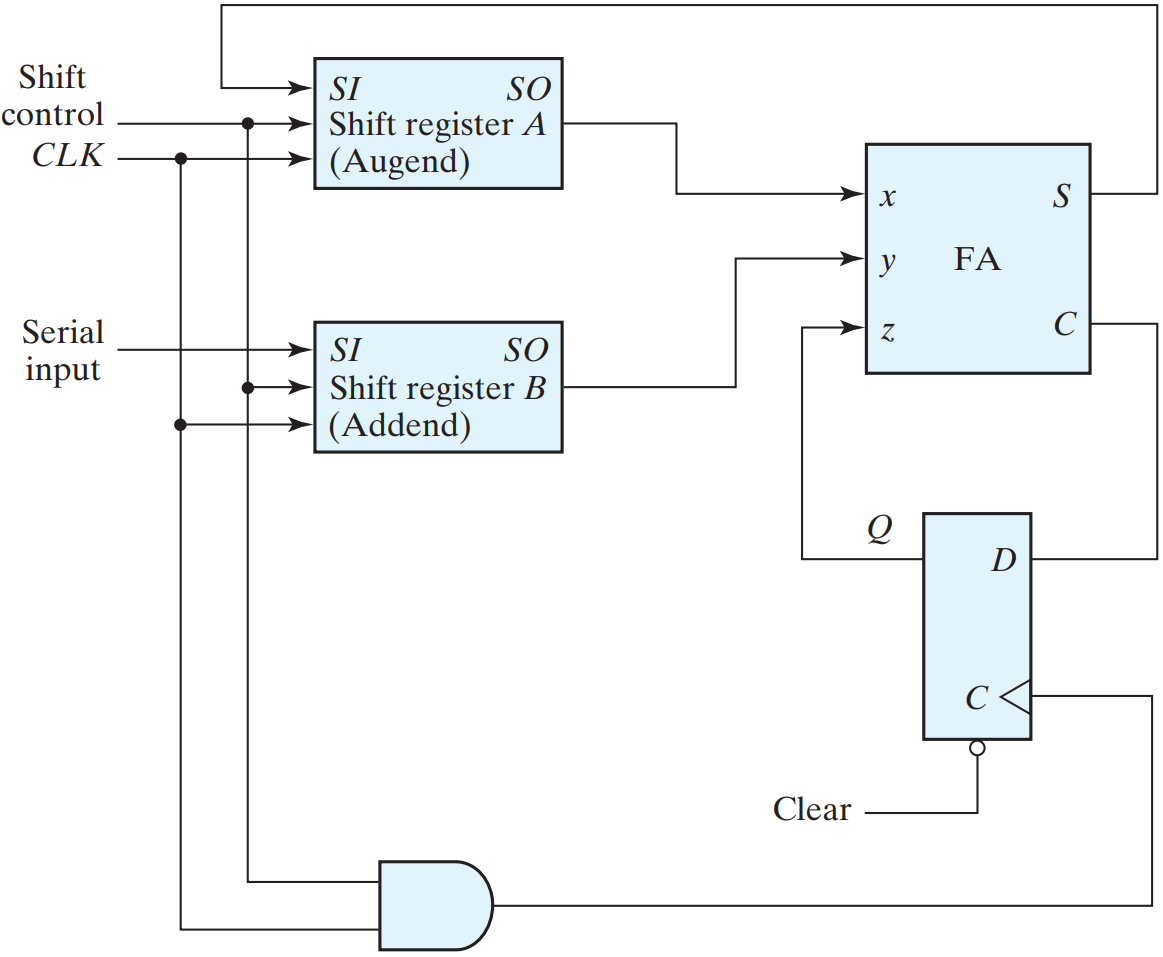
\includegraphics[width=\linewidth]{img/fig-6.5.png}
  \caption{Serial adder}
  \label{fig:6.5}
\end{figure}
Comparing the serial adder with the parallel adder, we note several differences.
\begin{itemize}
  \item The parallel adder uses registers with a parallel load, whereas the serial adder uses shift registers.
  \item The number of full-adder circuits in the parallel adder is equal to the number of bits in the binary numbers, whereas the serial adder requires only one full-adder circuit and a carry flip-flop.
  \item Excluding the registers, the parallel adder is a combinational circuit, whereas the serial adder is a sequential circuit, which consists of a full adder and a flip-flop that stores the output carry.
\end{itemize}

\noindent \textbf{Serial Adder with JK Flip-Flop:}
\begin{figure}[H]
  \centering
  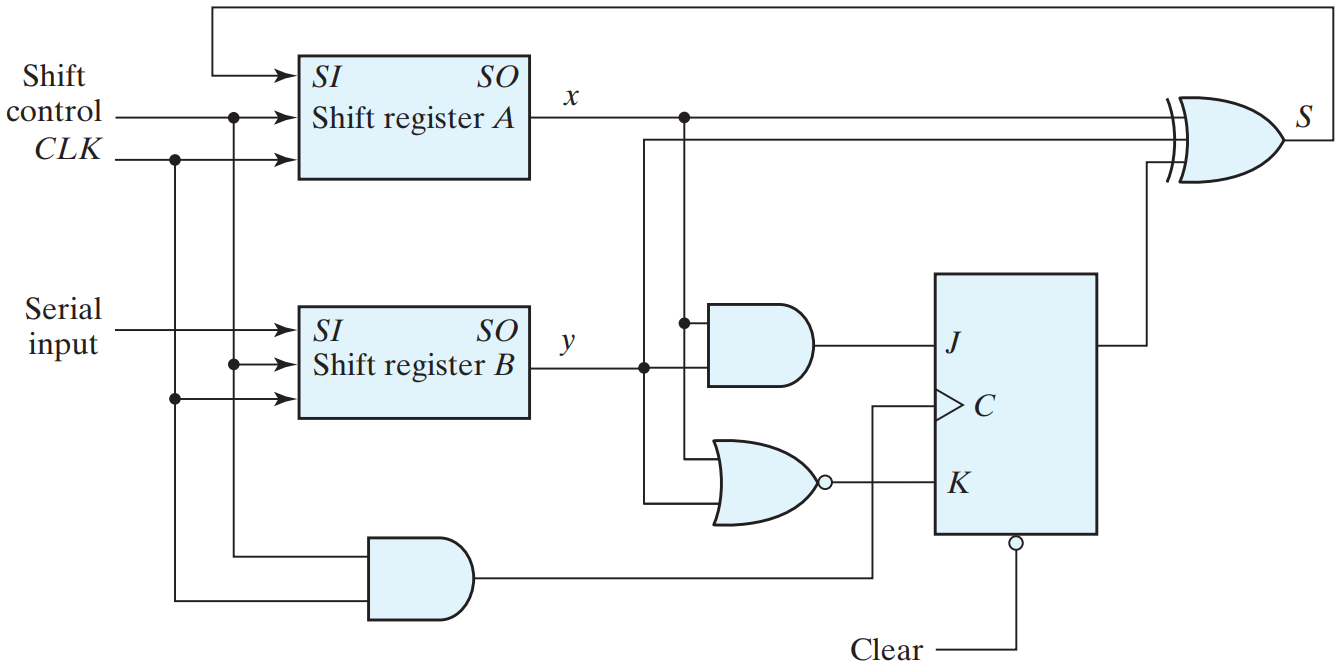
\includegraphics[width=\linewidth]{img/fig-6.6.png}
  \caption{Serial adder}
  \label{fig:6.6}
\end{figure}

\vspace*{\fill}
\columnbreak

\subsection{Universal Shift Register}
\label{subsec:universal-shift-register}

Some shift registers provide the necessary input and output terminals for parallel transfer. They may also have both shift-right and shift-left capabilities. The most general shift register has the following capabilities:
\begin{enumerate}[leftmargin=0.7cm]
  \item A \textit{clear} control to clear the register to 0.
  \item A \textit{clock} input to synchronize the operations.
  \item A \textit{shift-right} control to enable the shift-right operation and the \textit{serial input} and \textit{output lines} associated with the shift right.
  \item A \textit{shift-left} control to enable the shift-left operation and the \textit{serial input} and \textit{output lines} associated with the shift left.
  \item A \textit{parallel-load} control to enable a parallel transfer and the $n$ input lines associated with the parallel transfer.
  \item $n$ parallel output lines.
  \item A control state that leaves the information in the register unchanged in response to the clock.
\end{enumerate}

If the register can shift in both directions and has parallel-load capabilities, it is referred to as a \textit{universal shift register}.

The block diagram symbol and the circuit diagram of a four-bit universal shift register that has all the capabilities just listed are shown in Fig. 7. The circuit consists of four $D$ flip-flops and four multiplexers. The four multiplexers have two common selection inputs $s_1$ and $s_0$.

\begin{figure}[H]
  \centering
  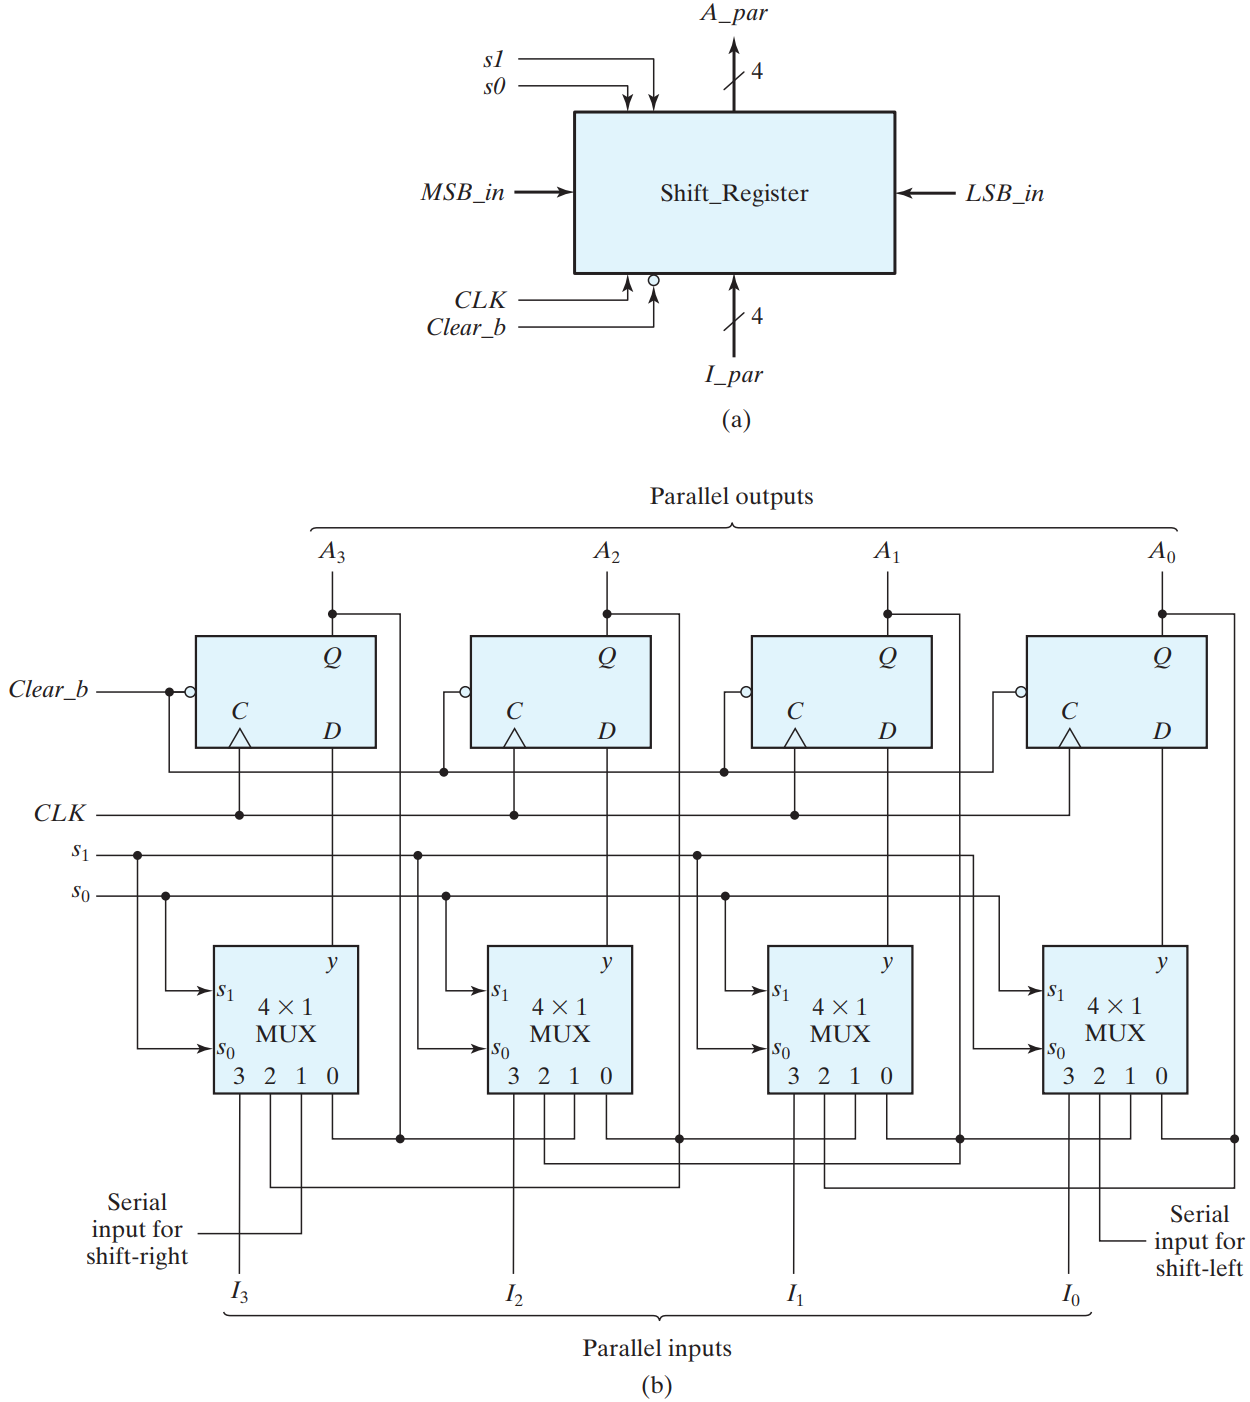
\includegraphics[width=\linewidth]{img/fig-6.7.png}
  \caption{Four-bit universal shift register}
  \label{fig:6.7}
\end{figure}

\vspace*{\fill}
\columnbreak

\begin{figure}[H]
  \centering
  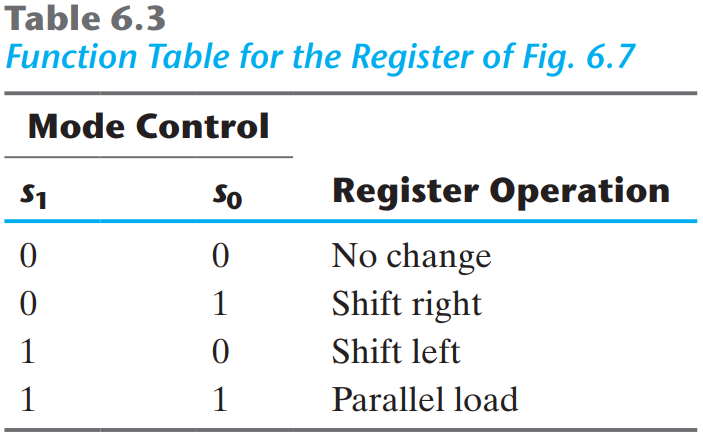
\includegraphics[width=\linewidth]{img/table-6.3.png}
  \label{table:6.3}
\end{figure}

\noindent\rule{\linewidth}{1pt}

\begin{figure}[H]
  \centering
  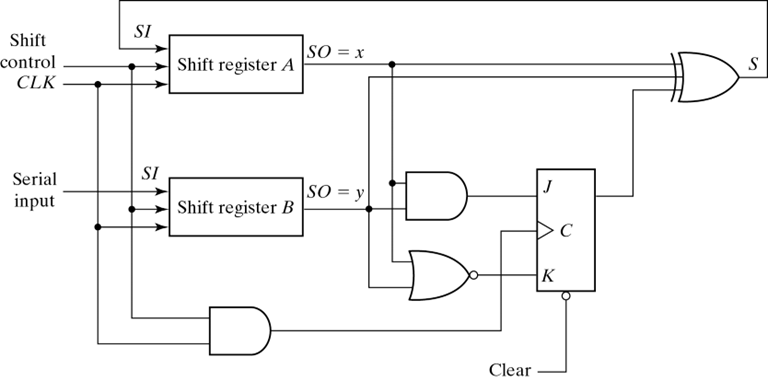
\includegraphics[width=\linewidth]{img/serial-adder-with-JK-FF.png}
  \caption*{Serial Adder with $JK$ Flip-Flop}
  \label{fig:serial-adder-with-jk-ff}
\end{figure}
